% Zusammenfassung und Ausblick
%

\lstdefinestyle{customc}{
  belowcaptionskip=1\baselineskip,
  breaklines=true,
  frame=L,
  xleftmargin=\parindent,
  %language=C,
  showstringspaces=false,
  basicstyle=\footnotesize\ttfamily,
  keywordstyle=\bfseries\color{green!40!black},
  commentstyle=\itshape\color{purple!40!black},
  identifierstyle=\color{blue},
  stringstyle=\color{orange},
}

\lstdefinestyle{customasm}{
  belowcaptionskip=1\baselineskip,
  frame=L,
  xleftmargin=\parindent,
  language=[x86masm]Assembler,
  basicstyle=\footnotesize\ttfamily,
  commentstyle=\itshape\color{purple!40!black},
}

\lstset{escapechar=@,style=customc}


\chapter{Results}

\section{Mouse brain model properties}

Three different circuits (see Table \ref{table:circuits}) are generated: The full mouse brain circuit,
a smaller circuit that contains 25 percent of the full mouse brain circuit and
$\frac{1}{300}$ of the full circuit. The percentage is related to the number of neurons inside
the circuit. The connections are generated based on the selection of neurons. In principle
number of connections should be of the same proportion as number of neurons.

\begin{table}[ht!]
\centering
%\begin{centering}
    \begin{tabular}{ | l | l | r | r | r |}
    \hline
    Identifier & ratio & neurons & synapses & total size \\ \hline \hline
    threehundredths & $0.3\%$ & $~2.5*10^5$ & $~2.2*10^9$ & $~26$ GB \\ \hline
    quater & $25\%$ & $~1.9*10^7$ & $~1.6*10^{11}$ & $~4$ TB \\ \hline
    full & $100\%$ & $~7.5*10^7$ & $~6.6*10^{11}$ & $~16$ TB \\ \hline
    \end{tabular}
%    \end{centering}
    \caption{The circuits \emph{threehundredths}, \emph{quater} and \emph{full} were created for testing and debugging on different scales.
All circuits were generated with identical parameters, only the input neuron file varies.}

\label{table:circuits}
\end{table}

The generated full mouse brain circuit contains around 74 million neurons and 660 billion synapses.
The simulation uses 12 parameters from the neuron file.
The file contains further parameters which are used for the connection generation and visualization,
like coordinates and neuron classifications. In total the neuron file is around 9 GB.
The synapse file contains only essential parameters for the simulation.
There are five synapse parameter per connection. This results in 15 TB of data
for the long range connectivity and 600 GB for the short range connectivity.
Thus, the generated circuit contains around 16 TB of data and it is split in three HDF5
files (neuron file, long range synapses file and short range synapses file).
The properties of the smaller circuits are equivalent.

\section{Manipulation of circuit}

The connection generation implementations accept a set of command line arguments.
The arguments allow to influence the program execution.
All accepted arguments are listed in table \ref{tab:longrangeargs}.
Besides data path manipulations the voxel experiment assignment can be 
manipulated on different levels. The number of used experiments can be specified
and limited. The interpolation can be enabled and limited to a range.
Also, the available voxel information can be mirrored to the other hemisphere.
Apart from this, the voxel experiment assignment can be exported to a file.
This file can be manipulated externally and imported again.

The weights of all created synapses can be strengthened by a set factor.
This is necessary for reduces models.
\begin{table}[ht!]
\begin{centering}
    \begin{tabular}{ | c | l | p{7cm} |}
    \hline
    Argument & expected type & function \\ \hline \hline
    \emph{-e} & path & set path to file, which contains picked experiment ids \\ \hline
    \emph{-n} & path & path to input neuron file \\ \hline
    \emph{-h} & path &  output folder\\ \hline
    \emph{-s} & - &  save voxel information\\ \hline
    \emph{-l} & path &  load voxel information\\ \hline
    \emph{-o} & - &  enable voxel interpolation\\ \hline
    \emph{-x} & - &  enable mirroring of voxels\\ \hline
    \emph{-c} & integer & only use one experiment with given id \\ \hline
    \emph{-m} & integer & limit number of loaded experiments \\ \hline
    \emph{-d} & integer & limit search distance for voxel interpolation \\ \hline
    \emph{-i} & integer & strengthening of weights for each synapse \\ \hline
    \end{tabular}
    \caption{Long range generation arguments to influence program execution.}
    \label{tab:longrangeargs}
\end{centering}
\end{table}

The short range generation only accepts path manipulations and weight strengthening.
The arguments are listed in table \ref{tab:shortrangeargs}.
\begin{table}[ht!]
\begin{centering}
    \begin{tabular}{ | c | l | p{7cm} |}
    \hline
    Argument & expected type & function \\ \hline \hline
    \emph{-n} & path & path to input neuron file \\ \hline
    \emph{-h} & path &  output folder\\ \hline
    \emph{-i} & integer & strengthening of weights for each synapse \\ \hline
    \end{tabular}
    \caption{Short range generation arguments to influence program execution.}
    \label{tab:shortrangeargs}
\end{centering}
\end{table}

\section{NEST import module}

Only one simulation case (\ref{ambmusecase}) of the mouse brain model is used in this thesis for performance evaluations.
Never the less, more use-cases are possible with the given implementations.
In general the neuron load module can be used as the neuron create function
and the synapses load module can be as the neuron connect function (see \url{www.nest-simulator.org/neural_simulations}).
Further, the given circuit can be loaded and adapted (use offset or scaling factor for parameters).
Loaded neurons can be divided into subnets. 
The \emph{SLI} functionality allows to access these subnets.
Thus, the grouping performed with the subnet dataset is available for all \emph{SLI} functions.
Stimulus generator and \emph{Spikedetector} or \emph{Multimeter} can be used to stimulate
and observe specific neurons, respectively.
More use-cases are possible: For example the \emph{SLI} connect functions can be used to strengthening or weakening the connections between the two
parts of the circuit.

An example SLI script is listed below.
It loads neuron and synapses information from the specified files.
Set a stimulus to neurons and connects neurons to a Spikedetector.
The example is similar to the used use-case.
\begin{lstlisting}[label=sliSynapses,caption=Example importing synapses]
%% Load neurons
/model /aeif_cond_exp def
/subnet (subnet_wl) def
/names [(C_m) (Delta_T) (E_L) (E_ex)] def
/filepath (circuit/ptneu_brain.h5) def
/param_factor [1. 1. 1. 1.] def
/param_offest [0. 0. 0. 0.] def
model names param_factor param_offest subnet filepath H5NeuronCsX /offset Set

%% Load synapses
/model /tsodyks2_synapse def
/hdf5_names [(delay) (weight) (U0)] def
/nest_names [(delay) (weight) (U)] def
/param_facts [1. 1. 1.] def
/param_offset [0. 0. 0.] def
/filepath (circuit/syn.h5) def
offset model nest_names hdf5_names param_facts param_offset filepath H5SynapseTll

%% Set stimulus to neurons in subnet 1
1 GetLocalChildren { 
    dup << /I_e 2500.0 pA >> SetStatus
} forall

%% Create Spikedetector
/spike_detector Create /spikedetector Set


%% Connect neurons in subnet 2 with Spikedetector
2 GetLocalChildren { 
    dup spikedetector Connect
} forall

%% Simulate for 100 ms
100.0 Simulate
\end{lstlisting}

\section{Import neurons}
The import neuron module can be executed with the function \emph{SLI} function  \emph{H5NeuronCsX}. It loads all neurons with its parameters
from the given HDF5 file. The function expects 4 input parameters:
\begin{itemize}
      \item Name of the a subnet dataset (String).
The subset has to contain for each neuron an integer value.
The neurons are grouped together by this subnet value.
      \item A list of all datasets which values are interpreted as list of parameters.
      
     
      \item Name of the used neuron model
      \item A list of dataset/parameter names, which are loaded from the hdf5 file and written to the neuron model
      \item A list of factor: The parameters are multiplied by the values
      \item A list of offsets: The parameters are increased by the values
      \item Name of the a subnet dataset (String).
The subset has to contain for each neuron an integer value.
The neurons are grouped together by this subnet value.
      \item path to the hdf5 file
\end{itemize}
It returns the neuron id of the first neuron is created.
\begin{figure}[ht!]
\begin{lstlisting}[label=sliNeurons, caption=Example usage of the import neuron module]
/model /aeif_cond_exp def
/subnet (subnet_wl) def
/names [(C_m) (Delta_T) (E_L) (E_ex)] def
/filepath (circuit/ptneu_brain.h5) def
/param_factor [1. 1. 1. 1.] def
/param_offest [0. 0. 0. 0.] def
model names param_factor param_offest subnet filepath H5NeuronCsX /offset Set

\end{lstlisting}
\caption{Calling the neuron import module via H5NeuronCsX SLI command.
\emph{nmodel} defines the neuron model.
\emph{subnet} defines the name of the subnet dataset.
\emph{nparameters} defines the name of the parameters datasets.
\emph{param\_factor} specifies an factor for each parameter value.
\emph{param\_offset} specifies an offset for each parameter value.
\emph{filepath} defines the filepath to the hdf file.
\emph{offset} returns the id of the first neuron loaded.}
\end{figure}

\section{Import synapses}
The import synapse module can be executed with the \emph{SLI} function  \emph{H5SynapseTll}. It loads all synapses with its given parameters
from the given HDF5 file. The function expects 7 input parameters:
 
\begin{itemize}
      \item Offset of the neuron ids. Mostly it is equal to first neuron id returned by \emph{H5NeuronCsX}
      \item Name of the used synapse model
      \item A list of parameter names, which are overwritten by the loaded values
      \item A list of column names, where the parameter values are loaded from
      \item A list of factor: The parameters are multiplied by the values
      \item A list of offsets: The parameters are increased by the values
      \item path to the hdf5 file
\end{itemize}
\begin{figure}[ht!]
\begin{lstlisting}[label=sliSynapses, caption=Example usage of the import synapse module]
/model /tsodyks2_synapse def
/hdf5_names [(delay) (weight) (U0)] def
/nest_names [(delay) (weight) (U)] def
/param_facts [1. 1. 1.] def
/param_offset [0. 0. 0.] def
/filepath (circuit/syn.h5) def
offset model nest_names hdf5_names param_facts param_offset filepath H5SynapseTll
\end{lstlisting}
\caption{Calling the synapse import module with the
SLI command \emph{H5SynapseTll}
\emph{offset} sets the offset of the neuron ids.
\emph{synmodel} specifies the synapse model name.
\emph{hdf5\_names} specifies the loaded synapse parameters
\emph{nest\_names} specifies the related synapse model parameters.
\emph{param\_facts} specifies factors for the parameter values.
\emph{param\_offset} specifies offsets for the parameter values.
\emph{filepath} specifies the filepath to the hdf5 file.}
\end{figure}

\section{Full mouse brain simulation}
The full mouse brain simulation was executed successfully on six racks of the JUQUEEN system.
For the simulation the full mouse brain model is loaded with a synapse weight strengthening of $10$.
The strengthening increases the diffusion of activity.
It enables the activation most of the neurons.
\begin{figure}[ht!]
     \begin{center}
        \subfigure[$t_{sim}=6 ms$]{%
            \label{fig:sim1}
            %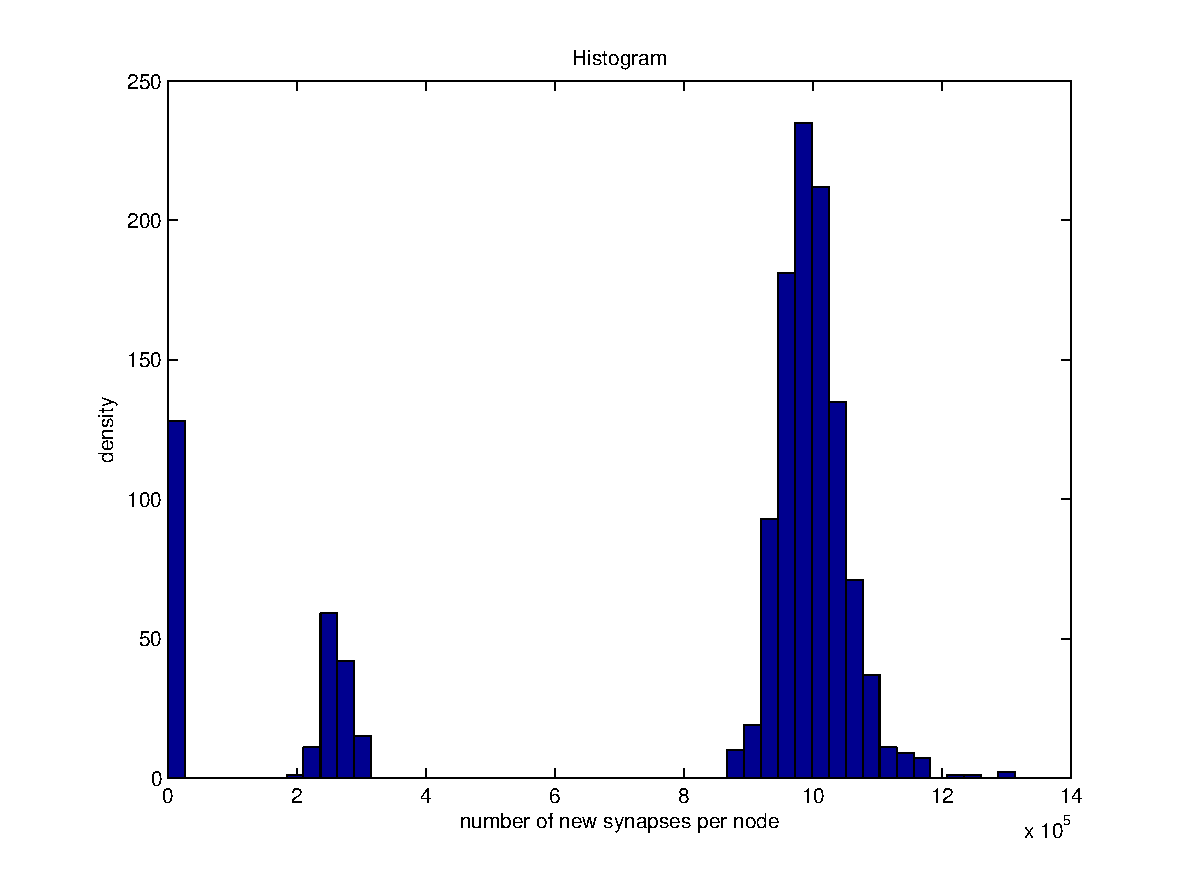
\includegraphics[scale=0.41]{pictures/histogram_new_const_1_300.eps}
            \includegraphics[scale=0.11]{pictures/vlcsnap-6ms.png}
        }
        \subfigure[$t_{sim}=18.5 ms$]{%
           \label{fig:sim2}
           %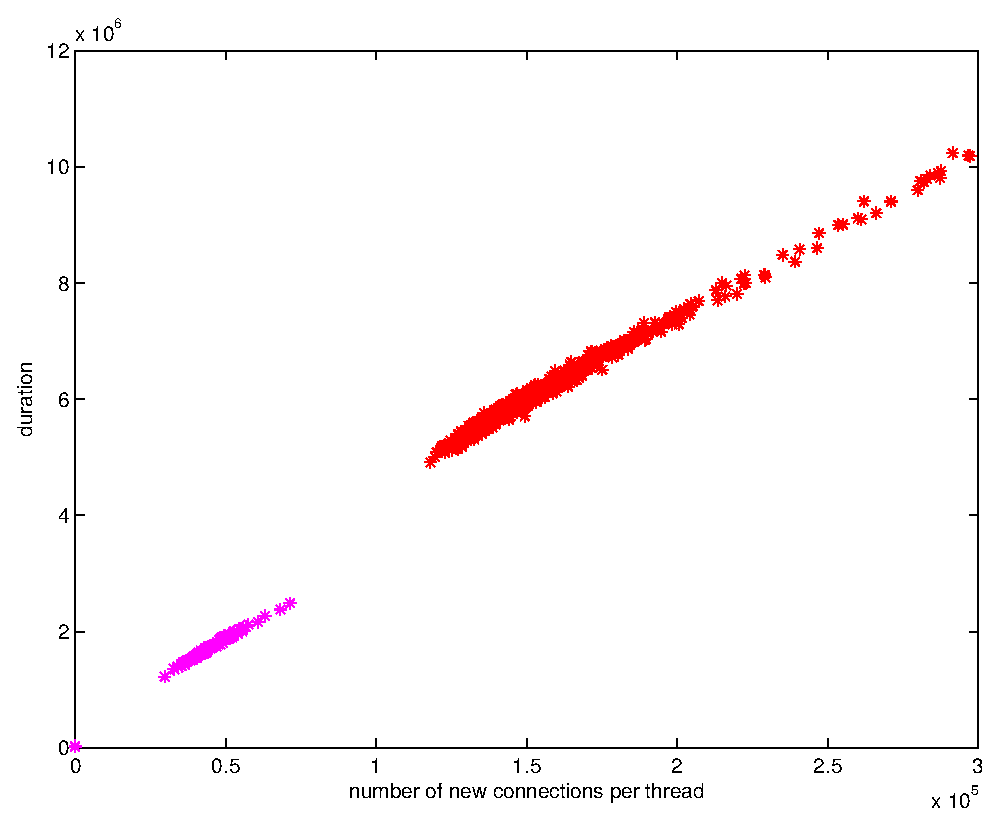
\includegraphics[scale=0.41]{pictures/t8_duration_per_con_1_300.eps}
           \includegraphics[scale=0.11]{pictures/vlcsnap-18ms.png}
		}
		\subfigure[$t_{sim}=19.5 ms$]{%
           \label{fig:sim2}
           %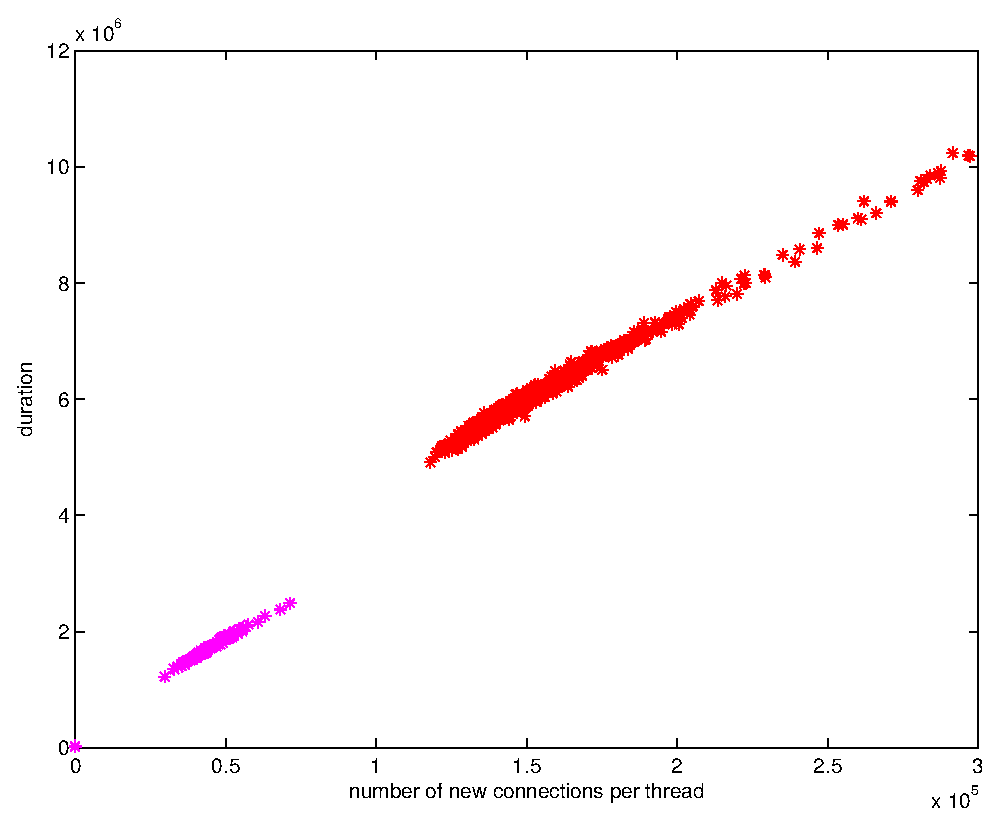
\includegraphics[scale=0.41]{pictures/t8_duration_per_con_1_300.eps}
           \includegraphics[scale=0.11]{pictures/vlcsnap-19ms.png}
		}
		\subfigure[$t_{sim}=25.8 ms$]{%
           \label{fig:sim2}
           %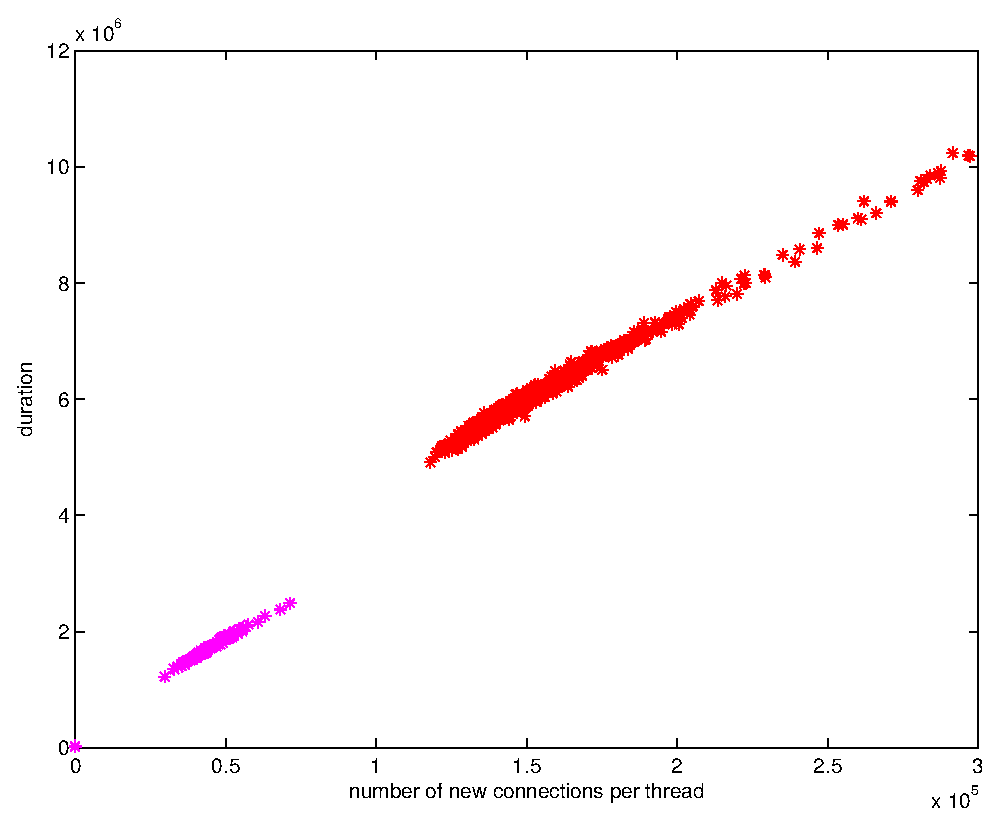
\includegraphics[scale=0.41]{pictures/t8_duration_per_con_1_300.eps}
           \includegraphics[scale=0.11]{pictures/vlcsnap-25ms.png}
		}
    \end{center}
    \caption{%
        Visualized spiking activity of a full mouse brain simulation.
        The figures show active neurons in four different time steps;
        Only active neurons are shown.
        The color represent the region of each neuron given by the Allen Brain Atlas.
     }%
   \label{fig:sim}
\end{figure}
The Figures \ref{fig:sim} show spiking activity for the given network.
Because of the strong strengthening the whole model excites and run into numerical errors
after a few milliseconds. But the run illustrates the possibility of the full mouse brain model
simulation. Even though the model is still under development, first experiments allow an insight 
into its behaviour.


\chapter{Discussion}
The generated model and the performance of the implementations are discussed.

\section{Mouse brain model extensions}
The given mouse brain model contained less synapses than there are in a living mouse.
To run a full mouse brain model anyway the circuit generation was extended by an interpolation.
The interpolation enables to generate a full mouse brain model from incomplete experimental data.
The interpolation, which are applied to the long range connection generation, introduces errors.
For illustration Figure \ref{interpolationdistance} shows the locality of missing voxels in one slice.
The quality of the interpolation can be estimated from distance between each voxel and the nearest injected voxel (color scale in Figure \ref{interpolationdistance}).
It highlights problematic regions.
\begin{figure}[ht!]
\centering
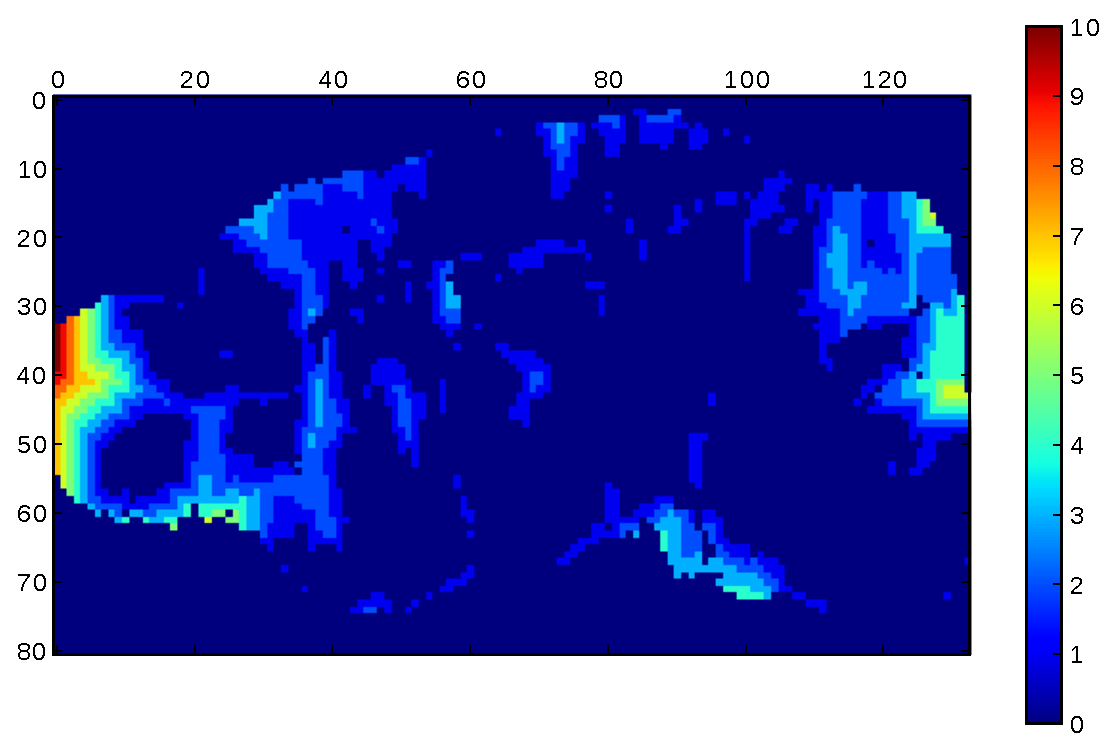
\includegraphics[scale=0.5]{pictures/distance_x_y_70.eps}
\caption{Plotted values from the nearest neighbor algorithm. One sees the distance to the next injected voxel.}
\label{interpolationdistance}
\end{figure}
The full mouse brain model can be loaded inside of NEST with the implemented modules.
If more experiments become available, they can easily be included into
the circuit generation. Further model properties are not discussed here.



\section{Data format usability}
The HDF5 data format for neuron parameters is used as received from the Neurorobotics team of the Blue Brain Project.
Because of the small size of the file (9 GB) in comparison to the synapse dataset (15 TB), the performance improvement by changing
to a transposed data format can be neglected. Thus, there is still advantage of having different datasets and being able
to add new datasets/parameters. It also implies that the generation script does not have to be converted and no 
conversion scripts are needed. The synapse data format focuses on an efficient storage of all essential values and parameters.
But the self descriptive format also allows a visualization and changes in the parameters.

\section{Long range connections generation}
Moving the best injection per voxel search outside the main iteration
avoids unnecessary calculations and reduces the complexity of the main iteration.
In the sequential algorithm, parts of the connections are regenerated in each iteration.
This is avoided by selecting the best injection per voxel beforehand.

Optimization of the linear acceptance rejection function (see \ref{par:linearacceptancerejection})
reduces the complexity of picking post-synaptic neurons.
For the full circuit this corresponds to a reduction of the complexity order  by two.
Using all core inside the function gives a further speed up.
Each thread has to pick $~\frac{10,000}{N_{threads}}$ voxels instead of
$10,000$.

The program execution takes around 15h on the Blue Brain IV using 2048 nodes generating the full circuit.
Each node uses all threads. Optimized collective writing operations could 
lower the needed execution time.
But is not feasible, because the generation script will be executed only a few times
and the computational resources are given.

\section{Short range connections generation}
We ported the sequential algorithm directly to a parallel implementation without changing it.
We introduce a Master-Slave aprraoch to mange the work distribution.
It enables an easy distribution of the independent iterations.
The critical part of the implementation is the IO because the number of created synapses is not known in the beginning.
Therefore, the file size cannot be calculated beforehand, which is mandatory for an efficient writing to HDF5 files. 
By using a buffer or temporary files this problem can be avoided.
Because of the given resources (Blue Brain IV)
writing all synapses to buffer is feasible (already for a small number of nodes the created synapses fit in memory).
The buffer implementation, which behaves like a queue, is efficient in terms of writing to disk and writing to file
if the queue chunks are large enough. Using larger chunks leads to 
a higher utilization of the theoretical bandwidth. Additionally, it leads to less independent
write operations which reduces the waiting time in serialization mechanisms.

The program execution takes around half an hour on the Blue Brain IV using 256 nodes for the full circuit.
Two MPI ranks per node are launched. Optimizing the load balance could lead a better performance.
But is not feasible, because the generation script will be executed only a few times
and the computational resources are given.

\section{Import circuit}
Loading the mouse brain model inside of NEST is the main goal of the thesis.
Therefore, NEST is extended with two import modules, which enable to import the
generated mouse brain model. To show that the implemented algorithms are feasible, 
the circuit properties which affect the load balance, are analysed.
The synapse import module has to load around 15 TB of data for the full mouse brain model.
The neuron import module has to load only 9 GB of data.
Therefore, only the efficiency of the synapse import module is analysed.
Timings of the neuron import module are negligible.
The performance characteristics of the implemented algorithm is presented.
The IO performance of the implementation affects mainly the usability.
Runs on different scales should give detailed information about the reached bandwidth.
Therefore, IBM Blue Gene /Q systems in Lugano (Blue Brain IV) and in J\"{u}lich (JUQUEEN) are used.

During development the connect step was identified as the bottleneck.
Therefore, we introduced thread parallelism of the \emph{connect} step (see Section \ref{sec:speedup:connect}).
By the following measurements these optimizations are applied.

In the course of a scalability workshop in Forschungszentrum J\"{u}lich we were able to run
our implementation on different scales of JUQUEEN.
Findings of the \emph{Read} step gotten from the workshop are presented in \ref{sec:speedup:load}.
Optimizations are not included inside the implementation yet.
Therefore, they are not part of the measurements.
\begin{table}[ht!]
\begin{center}
\begin{tabular}{|l|l|l|p{1.9cm}|p{2.1cm}|l|}
\hline
name & scaling & importing & mpi ranks per node & threads per mpi rank & racks \\
\hline\hline
First    &  strong  & $1.9$ $TB$             & 1 & 16 & 1, 2, 4, 8, 16, 28 \\
Second    &  weak  & $900$ $\frac{MB}{node}$      & 1 & 16 & 1, 2, 4, 8, 28 \\
Third    &  weak  & $220$ $\frac{MB}{node}$     & 1 & 16 & 1, 2, 4, 8, 16, 28 \\
\hline
\end{tabular}
\end{center}
\caption{Properties of scaling runs}
\label{schumann:tbl:runs}
\end{table}

Two weak scaling and one strong scaling scenarios were tested on the JUQUEEN.
Therefore, the total time of executing the synapse import module were measured.
The properties of the scaling runs are listed in table \ref{schumann:tbl:runs}.

The amount of data read in the import module depends on the number of synapse parameters $N_{params}$,
the number of read synapses per iteration $N_{blocksize}$ and the number of ranks $N_{ranks}$.
This results in a measured bandwidth of:
\begin{equation}
b = sizeof(float) * N_{params} * \frac{N_{blocksize} * N_{ranks}}{\Delta T}
\label{eq:band}
\end{equation}
We use the equation \ref{eq:band} to normalize the scaling runs.
\begin{figure}[h!]
\begin{center}
 \includegraphics[width=0.8\textwidth]{pgfplots/bandwidth.pdf}
\end{center}
\caption{Bandwidth comparisons at different scales (see table \ref{schumann:tbl:runs}).
The plotted values are taken from Table \ref{schumann:tbl:scalruns}.
The \emph{theoretical} line shows the approximate bandwidth peak of the system.}
\label{schumann:fig:bandwidth}
\end{figure}

Figure \ref{schumann:fig:bandwidth} plots the measured bandwidth for the runs over number of nodes.
The resulted bandwidths tackles around $5\%$ of the peak bandwidth.
All runs give similar results. The difference of strong versus weak scaling runs seems to be negligible.
The amount of data, which is loaded does, not influence the results, as well.
The reached bandwidth only correlates with the number of racks.
For both IBM Blue Gene /Q systems the number of IO nodes scales linear with the number of racks.
Therefore, we cannot conclude if the number of IO nodes or the number of nodes limit the
bandwidth.

A more detailed look on the task scale should give more insights.
An instrumented version of the implementation with scorep gives us wall-clock timings of each task.
The tasks are \emph{Read}, \emph{Def. Node}, \emph{Sort}, \emph{Alltoall} and \emph{Connect} and relate to the main 
parts of the algorithm (see Figure \ref{fig:ConnectInsideIteration}).
We execute the instrumented module on different scales.
We analyse the measurements with Scalasca (see Appendix \ref{appendix:scalasca}).
The runtime behaviour is similar, of all runs.
The duration of \emph{Sort} and \emph{Det. Sort} is constant.
It depends on the buffer size, which is fixed for all runs.
Therefore, we can neglect the steps for the analysis.
For illustration, we present the runtime proportion of each task for the 1st scaling runs.
The mean percentage for each tasks over all nodes is calculated (see Figure \ref{schumann:fig:taskratios}).
\begin{figure}[h!]
\begin{center}
 \includegraphics[width=0.5\textwidth]{pgfplots/taskratios.pdf}
\end{center}
\caption{Measured task durations percentages of the total duration at different scales.
 The displayed percentages are the means of percentages for all nodes.
 The values are extracted from the 1st scaling run (see table \ref{schumann:tbl:runs}).
 }
\label{schumann:fig:taskratios}
\end{figure}

\emph{Read} and \emph{Alltoall} take most of the time at all scales.
Comparing the proportions with Figure \ref{schumann:fig:bandwidth}, we conclude that
\emph{Det. Node}, \emph{Sort} and \emph{Connect} scale approximately linear with the number of racks.

\begin{table}[h!]
\begin{center}
\begin{tabular}{|r|r|r|r|r|r|r|r|}
\hline
racks & MPI ranks & 1st $T$ & 1st \emph{sib} & 2nd $T$ & 2nd \emph{sib} & 3rd $T$ & 3rd \emph{sib} \\
\hline\hline
1  & 1024      & 1222 & 80640M & 523 & 40320M & 123 & 8960M \\
2  & 2048      & 642 & 80640M  & 593 & 80640M & 118 & 17920M\\
2  & 4096      & 363 & 80640M  & 661 & 161280M & 139 & 35840M\\
4  & 8192     & 325 & 80640M & 827 & 322560M & 245 & 71680M \\
8  & 16384    & 208 & 80640M & -   & - &  364 & 143360M \\
16  & 28672    & 168 & 80640M & 1401 & 1128960M & 497 & 250880M\\
\hline
\end{tabular}
\end{center}
\caption{Scaling runs of the import module using independent read calls on JUQUEEN. \emph{1st $T$} and \emph{sib}, \emph{2nd $T$} and \emph{sib} and
  \emph{3rd $T$} and \emph{sib} corresponds to the wall-clock timings and number of synapses for the First, Second and Third scaling runs (see table \ref{schumann:tbl:runs}). \emph{M} equates an factor of $2^{20}$ for number of synapses. On each rack $1024$ nodes are used.}
\label{schumann:tbl:scalruns}
\end{table}

%\subsection{Load balance}
%The neurons are distributed equably on all processes based on equation \ref{eq:processfromid}.
%But the number of incoming synapses varies between the neurons.
%Therefore a memory imbalance could occur between the processes.
%To analyse the imbalance, an analysing script iterates over the \emph{syn} dataset and counts
%the number of incoming synapses per neuron. Normalized results are plotted in box-plot diagrams 
%in Figure \ref{fullcircuitdist}.
%It shows an increasing imbalance of synapses per process with increasing number of processes.
%\begin{figure}[ht!]
%\centering
%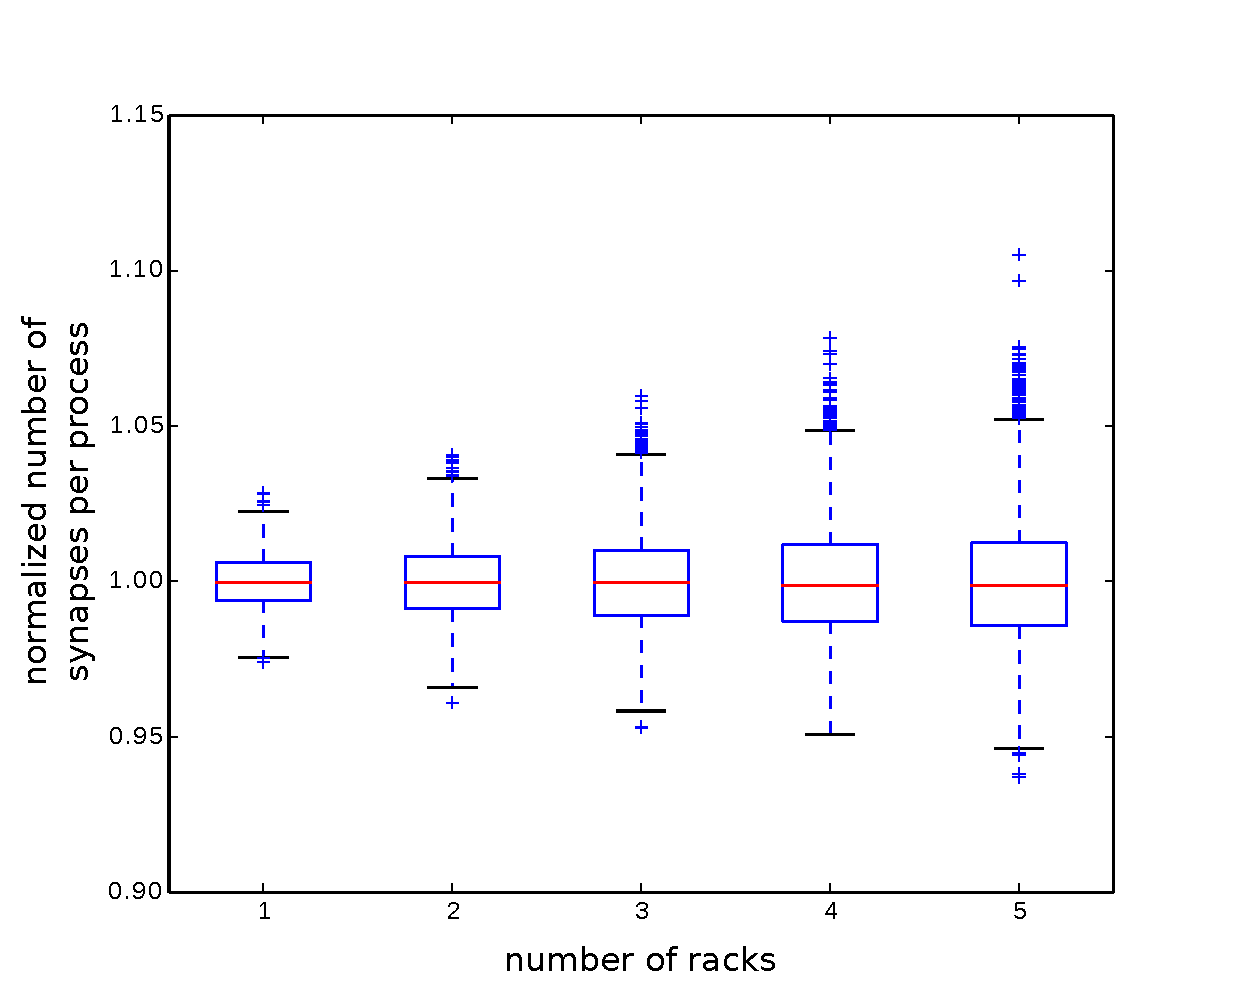
\includegraphics[scale=0.4]{pictures/full_circuit_rack_distribution.eps}
%\caption{Estimated synapse imbalance of neuron distribution on processes.
%It shows the distributions of relative sums (sum of number of synapses per process divided by %mean of sums) of synapses per process (y-scale) on different scales (x-axis). Relative sums %means absolute sums devided by the mean sum per process. }
%\label{fullcircuitdist}
%\end{figure}


%\begin{figure}[ht!]
%     \begin{center}
%        \subfigure[Load hdf5 files]{%
%            \label{fig:first}
%            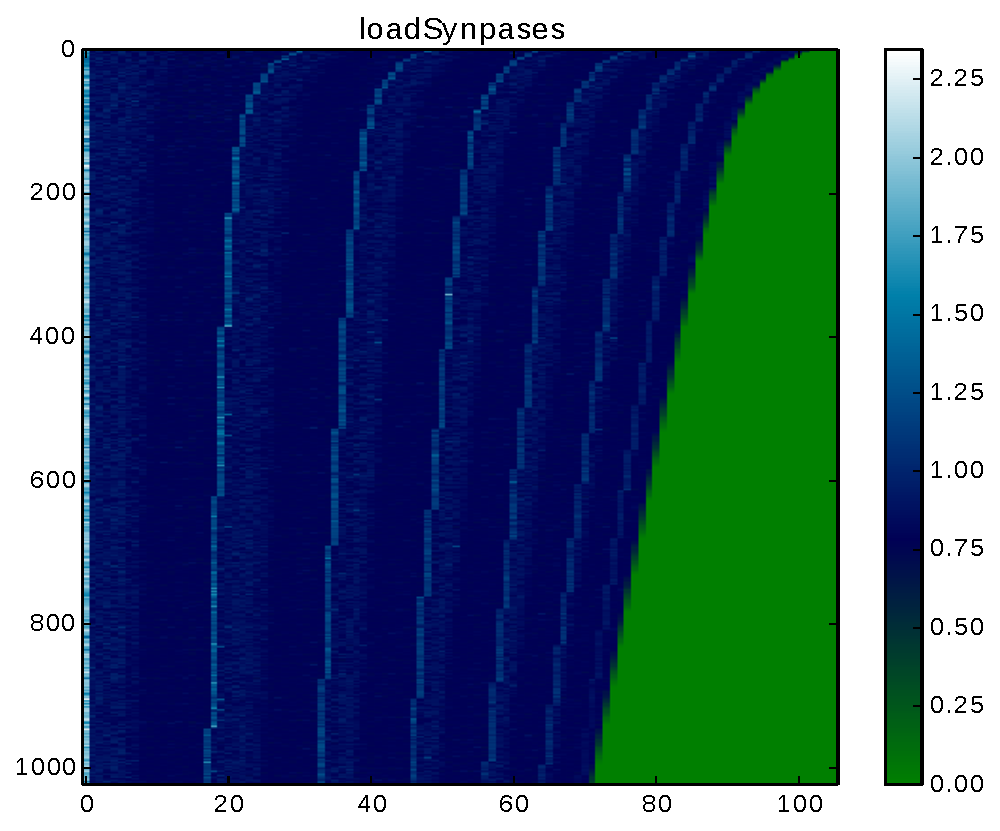
\includegraphics[width=0.45\textwidth]{pictures/V03_loadSynapses.eps}
%        }
%        \subfigure[Sort connection information data by target node]{%
%           \label{fig:second}
%           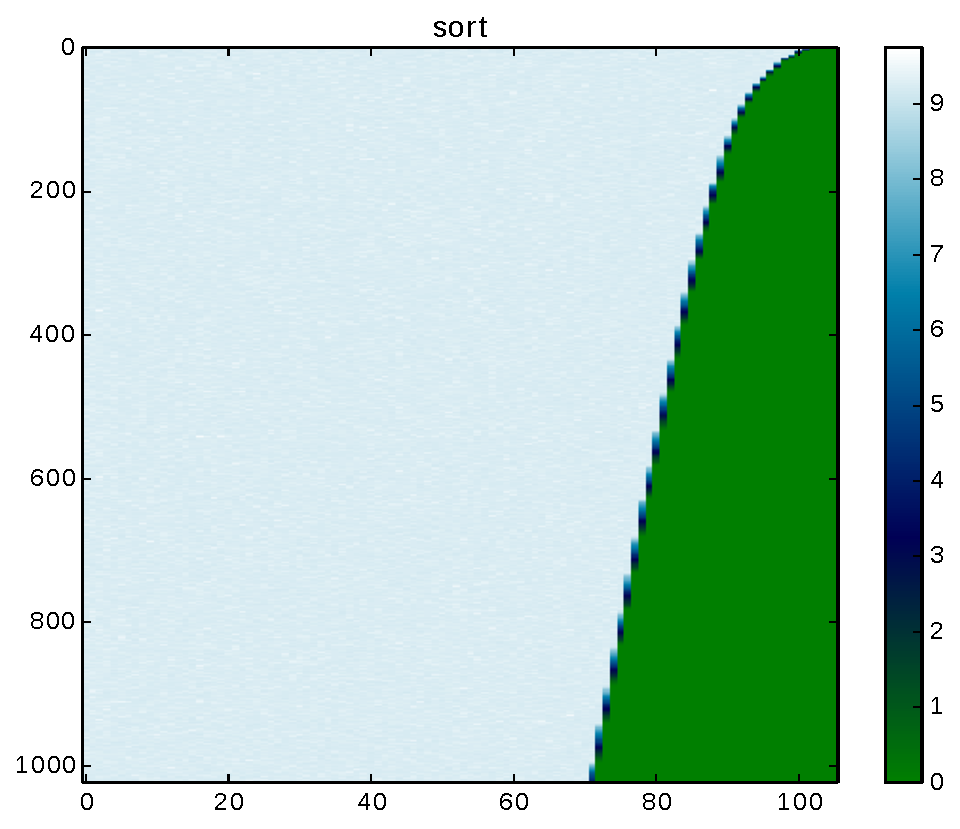
\includegraphics[width=0.45\textwidth]{pictures/V03_sort.eps}
%        }\\ %  ------- End of the first row ----------------------%
%        \subfigure[Send data to all target nodes using AlltoAllv]{%
%            \label{fig:third}
%            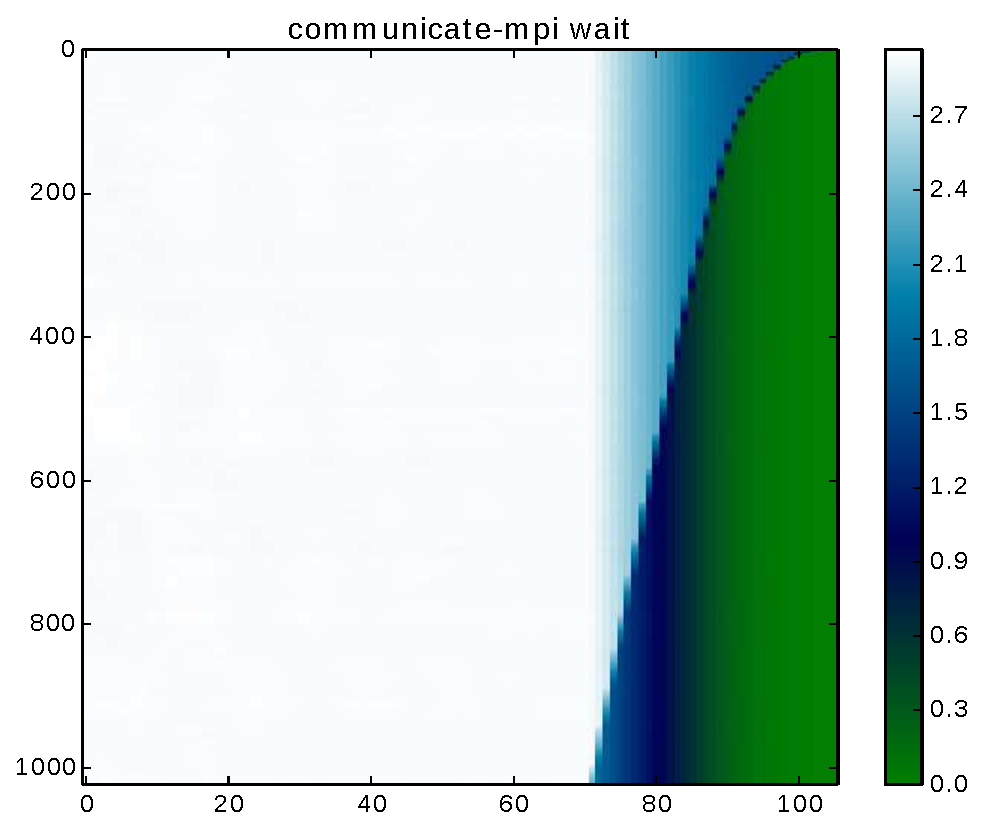
\includegraphics[width=0.45\textwidth]{pictures/V03_communicate.eps}
%        }
%        \subfigure[Connect function which calculated delay and calls NEST connect]{%
%            \label{fig:fourth}
%            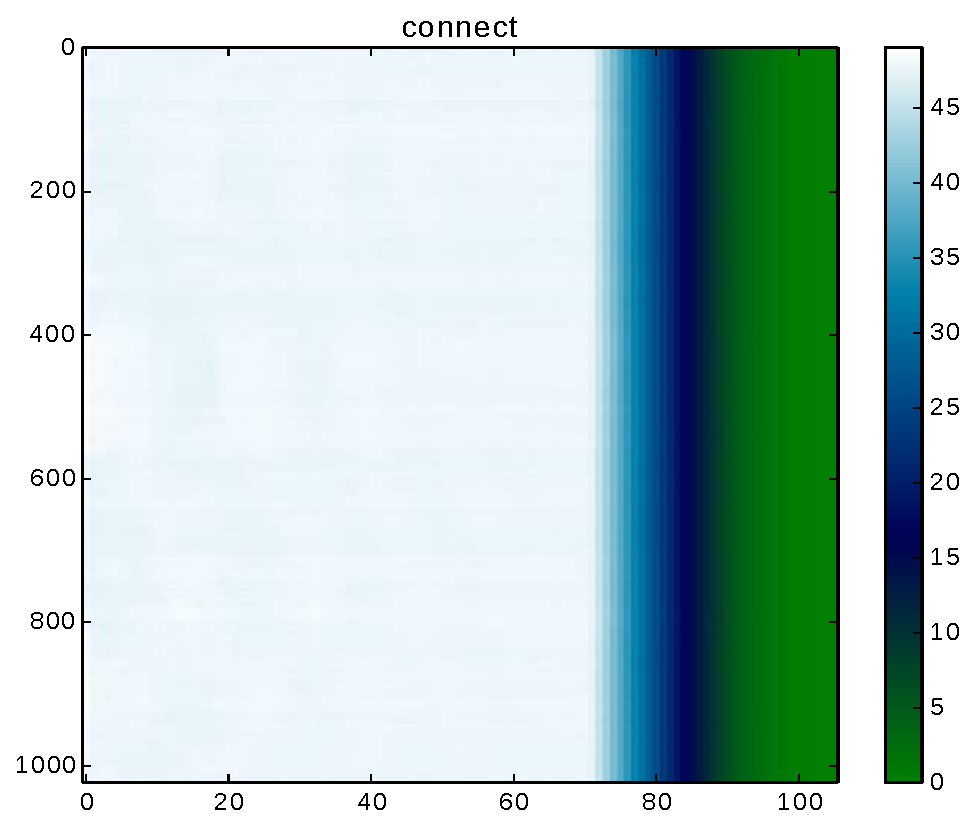
\includegraphics[width=0.45\textwidth]{pictures/V03_connect.eps}
%        }
%    \end{center}
%    \caption{%
%        The the plots show the the execution time for node per iteration.
%        The y-axes corresponds to the node id and the x-axes corresponds to the iteration number.
%        The color scale is in seconds.
%        In each iteration loadSynapses loads max $1e6$ synapses from hdf5 file.
%     }%
%   \label{fig:implV03}
%\end{figure}
One can see that \emph{Read} and \emph{Connect} are the bottlenecks.
For the interpretations of the plots, one has to take into account that different parts of the algorithm
(\emph{Read} and \emph{Alltoall}) contain mpi collective operations.

\subsection{Read step}
\label{sec:speedup:load}
The efficiency of the \emph{Read} step is bounded by the IO bandwidth of the system.
Blue Brain IV and JUQUEEN have a theoretical bandwidth of $8$ GB/s per rack.

Apparently, \emph{Read} and \emph{Alltoall} affect mainly the run time of our module.
\emph{Read} performs io. It uses the HDF5 library to load synapses from disk to the internal data structure.
\emph{Alltoall} exchanges synapses between the ranks. Both tasks contain collective MPI calls.
A detailed look at the call stack of the used H5Read function shows that the called MPI read operation is non-collective.
Using the HDF5 property list interface, we identify that the internal data structure of the import module prevents HDF5 from using collective read operations.
A collective read operation could result in better read performance.
Therefore, a comparison of collective versus independent read operations should show possible benefits.
Because of the limited time at the workshop, we focus on the comparison of a reduced algorithm,
which allows an easy change of the used data structure.
We can provide two test implementations with and without adapted data structure.
\begin{figure}[h!]
\begin{center}
 \includegraphics[width=0.8\textwidth]{pgfplots/bandwidth_stats.pdf}
\end{center}
\caption{Comparison of achieved bandwidth from collective versus independent read operations.
 Values from table \ref{schumann:tbl:indevscol} are used. Theoretical line shows the limits by the
 JUQUEEN system.}
\end{figure}
The new algorithm reduces the iterations to the \emph{Read} part with a following MPI barrier.
The MPI barrier should simulate any \emph{collective} read operations inside the \emph{alltoall} task.
\begin{figure}[h!]
\begin{center}
 \includegraphics[width=0.5\textwidth]{pgfplots/indiVScollec.pdf}
\end{center}
\caption{Comparison of collective versus independent read operations executed on 16 racks.
 Values are extracted from the scorep measurements from the runs listed in table \ref{schumann:fig:indiVScollec}.}
 \label{schumann:fig:indiVScollec}
\end{figure}

\newpage
Figure \ref{schumann:fig:indiVScollec} illustrates the benefit of collective versus independent read operations
on the JUQUEEN system for 16 racks.
Even though the mean time of the read operations is similar, the serializations of the read calls affects the
imbalance and therefore the idle times at the next collective operations. 
Therefore, a change in the data structure should bring great benefit for our implementation.
We are confident that the optimization will result in better usage of the available bandwidth.

\begin{table}[h!]
\begin{center}
\begin{tabular}{|r|r|r|r|r|r|}
\hline
racks & MPI ranks & mpiio & synapses in buffer & time[s] \\
\hline\hline
2  & 2048      & independent  &  8960M & 36.7041712582\\
4  & 4096      & independent  & 8960M  & 21.6904791038\\
16  & 16384      &  independent & 286720M  & 406.885908909\\
0.5  & 512      & collective  & 8960M  & 70.67277588\\
2  & 2048      & collective  & 8960M  & 29.0894202424\\
4  & 4096      & collective  & 8960M  & 12.5637469038\\
8  & 8192      & collective  &  8960M & 7.9934176194\\
16  & 16384      &  collective & 286720M  & 191.27968665\\
\hline
\end{tabular}
\end{center}
\caption{Scaling runs of test implementation to compare collective versus independent read calls on JUQUEEN. \emph{bytes~per~synapse} is $24$ for all runs.
  \emph{M} equates an factor of $2^{20}$ for number of synapses. On each rack $1024$ nodes are used.}
\label{schumann:tbl:indevscol}
\end{table}
\subsection{Alltoall step}
The \emph{Alltoall} step contains collective MPI communications.
Inside, \emph{MPI\_alltoall} is called followed by \emph{MPI\_alltoallv}.
The Scalasca analysis highlights the first \emph{MPI\_alltoall} as the bottleneck,
even though the second \emph{MPI\_alltoallv} transfers more data.
This means, that the internal MPI barrier is responsible for the bottleneck.
Thus, it can be traced back to imbalance resulting from the independent read operations.

\subsection{Connect step}
\label{sec:speedup:connect}
Thread parallelization of the connect step allows to store the synapses efficiently in the NEST data structure.
The pure connect functionality of NEST is thread-safe. But creating and destroying SLI data objects is not and can result
in data-races. To overcome this limitation, the creation and destroying of the objects is serialized.
Before iterating over all synapses, one SLI object is created and destroyed afterwards for each thread.
A single connect function call of the NEST api expects the synapse parameters stored in a SLI object.
In each iteration the current parameters are assigned to the values inside the already created SLI object.
This SLI object is passed to the function call.
Thus, a small overhead for the creation and destroying of the objects are perceived.
\begin{figure}[ht!]
\centering
%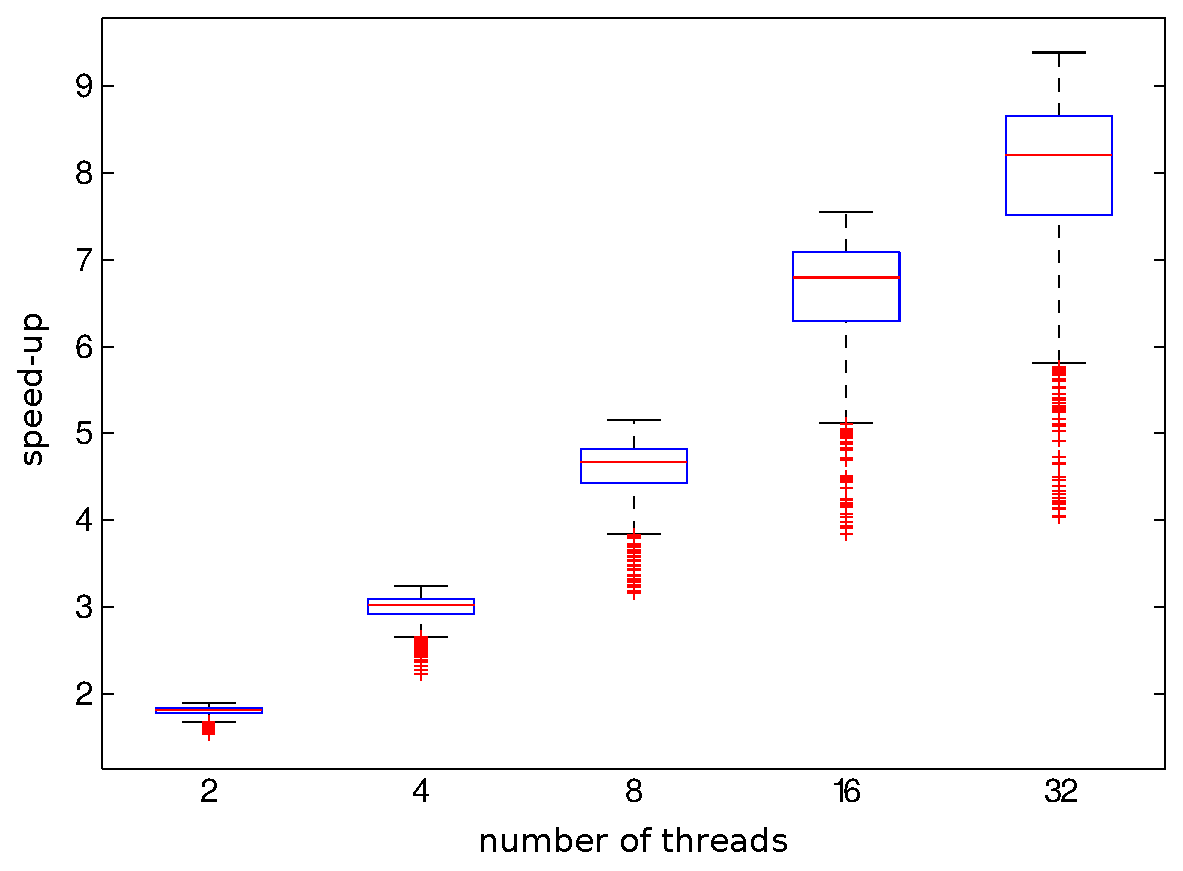
\includegraphics[scale=0.5]{pictures/boxplot_new_con_dt_1_300_speedup.eps}
\includegraphics[scale=1]{pgfplots/boxplot_thread.pdf}
\caption{The connection frequency per node for different number of threads is shown.
The plot shows boxplots of measured values using the threehundredths circuit.
The whiskers, the box boundaries and the middle lines represent the maximum outliers,
the 95/5 quantiles and the median values, respectively.
}
\label{boxplotnewcon}
\end{figure}
Each thread iterates over all synapses, but only stores the connection if the post-synaptic neuron is located on
the thread. Thus, the connection frequency per thread varies.
As for nodes the neurons are distributed in the modules fashion on the threads for one node.
The distribution properties are the same. Thus, there is a larger variation on a larger number of threads.
Figure \ref{boxplotnewcon} shows measured connection frequencies for the connect step. The measurements are
extracted from the execution of the threehundredths circuit. It is executed on 128 nodes with varying number of
threads. The circuit plus fixed number of nodes specify the distribution of neurons per node.

\begin{figure}[ht!]
     \begin{center}
        \subfigure[Histogram showing measured densities of number of new synapses per iteration step for one node.]{%
            \label{detailnewcon:first}
            %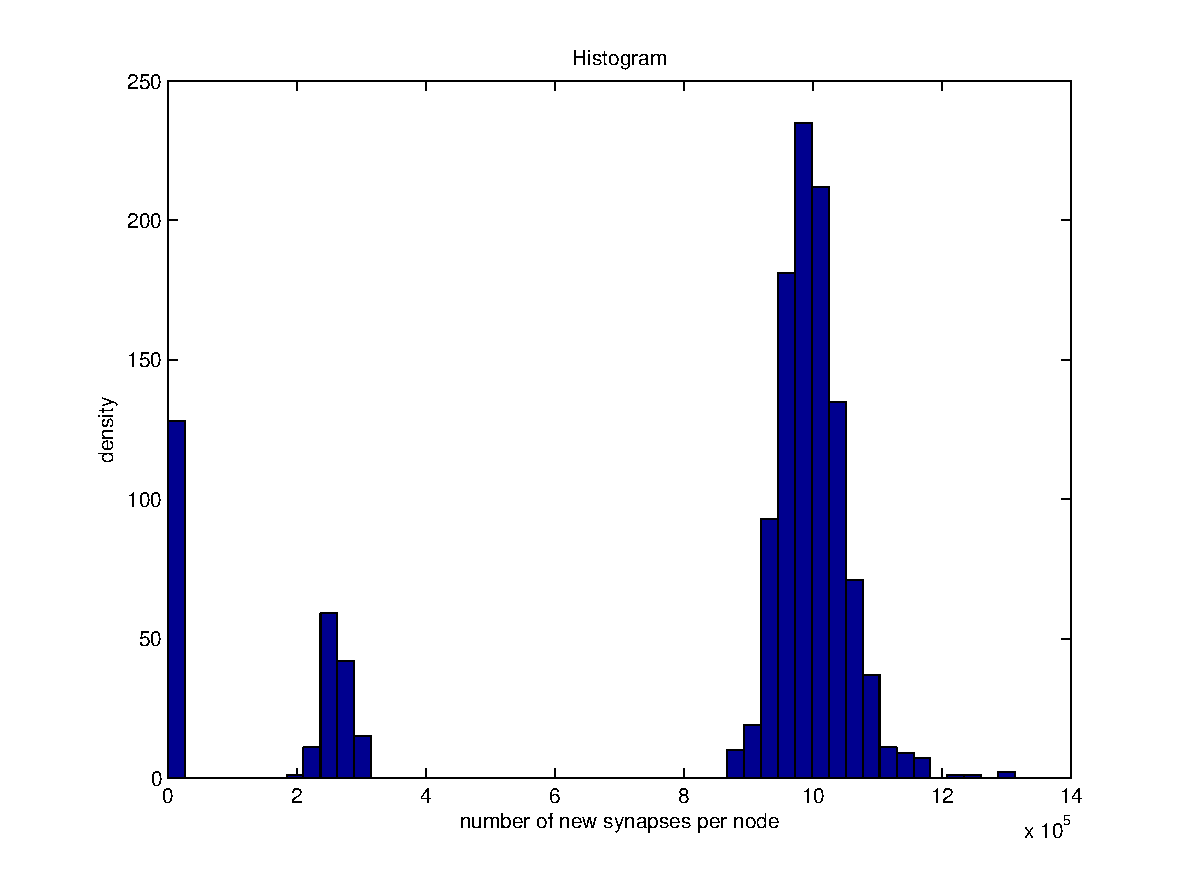
\includegraphics[scale=0.41]{pictures/histogram_new_const_1_300.eps}
            \includegraphics[scale=0.9]{pgfplots/histogram_num_syn.pdf}
        }
        \hspace{0.2cm}
        \subfigure[Plotted wall-clock timings of \emph{connect} step over the number of new synapses for one thread
        			(Thread is located on the node from Figure \ref{detailnewcon:first}. The new synapses are part of the new synapses from the node).
        			Red and green dotes relate to iterations, where the number of new synapses is smaller and bigger than $4*10^5$,
        			respectively (The values relate to the hills from Figure \ref{detailnewcon:first}). 
        			]{%
           \label{detailnewcon:second}
           %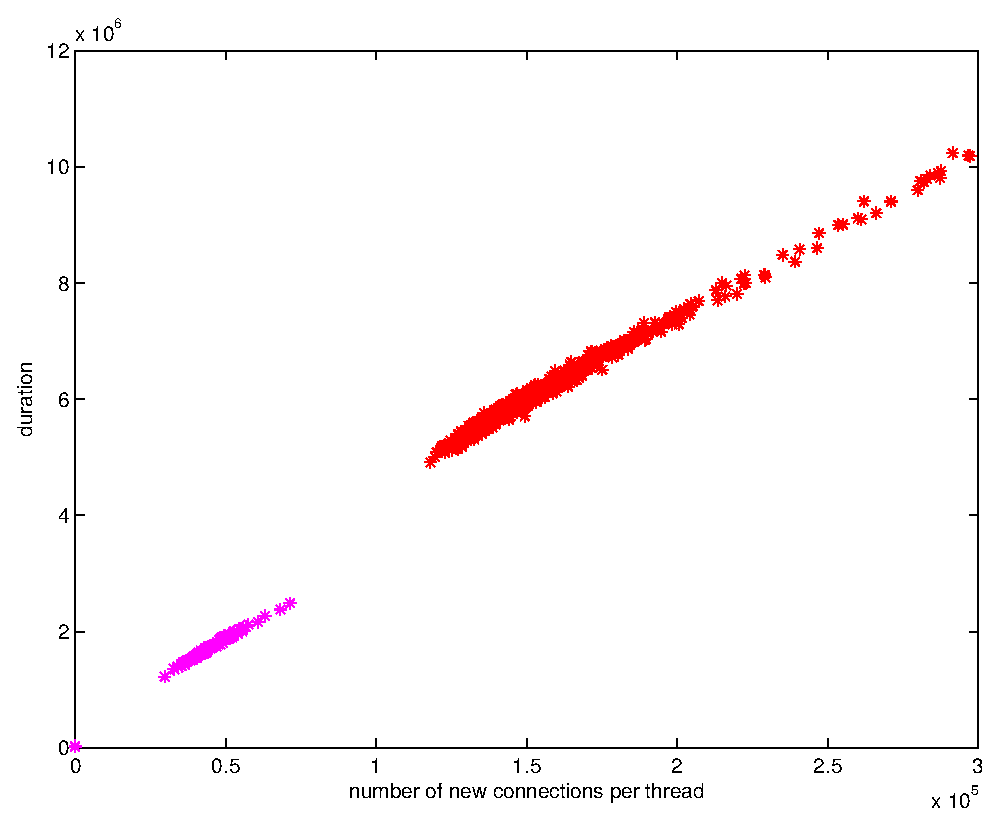
\includegraphics[scale=0.41]{pictures/t8_duration_per_con_1_300.eps}
           \includegraphics[scale=0.9]{pgfplots/connetions_thread.pdf}
		}
    \end{center}
    \caption{%
        The measurements are taken the same simulation run with the threehundredths circuit. It is run on the Blue Brain IV.
     }%
   \label{detailnewcon}
\end{figure}

A larger number of threads leads to smaller wall-clock timings, but the chance of imbalance increases.
%The variations of the timings correlates with the distribution of synapses per node (figure \ref{fullcircuitdist}).
To look into detail, Figure \ref{detailnewcon:second} shows the measured wall-clock time for each node
plotted over the maximum number of new connections per thread. It shows a strong correlation between the variable and
the duration. Thus, the increasing variations of timings can be explained by the variations of synapses per thread.
The figure indicates two different timings per connection. There is an offset of regression between the red
(left point cloud)
and the green (right point cloud) dots. Red and green dots represent all measurements with less than $40,000$ and more than new synapses per
node, respectively. Less than $40,000$ new synapses only occurs in the last iteration.
Figure \ref{detailnewcon:first} shows the density of number of new synapses per node.
Less synapses results in a smaller vector size. There seems to be a loss of efficiency, which might result from
the use of different cache levels.

\section{Memory consumption}
During the development of the import module, the goal to fit the full mouse brain model on the
Blue Brain IV seemed to get unrealistic. We make the assumption that the full machine does not deliver enough memory resources for the whole circuit.
Test runs on different scales on the JUQUEEN should give concrete results for the final implementation.
The test runs load the neuron information and the long range synapses.
The long range synapses are approximately 96\% of synapses in the full circuit.
Thus, reducing the test to only the long range synapses is feasible.
We extended the import module with a logging of imported synapses and the used memory after each iteration.
We used a BGQ library (see Appendix \ref{bgqmemory}) to measure the memory usage on each node.
The runs on $6$ and $8$ racks executed successfully.
The run on $4$ racks crashed before ending.
It run out of memory.
\begin{figure}[h!]
\begin{center}
 \includegraphics[width=0.9\textwidth]{pgfplots/newconnections.pdf}
\end{center}
\caption{Number of synapses in memory over iterations.
The solid, dotted and dashed lines represent the mean, minimum and maximum number of synapses in memory of all nodes, respectively.
The green lines show the measurements from a run on 8 racks, the blue on 6 racks and the red on 8 racks.
The points represent the last iteration per run.
Thus, the program iterates $80$ times on $8$ racks, $107$ times on $6$ racks and $140$ times on $4$ racks.
The numbers 1, 2 and 3 represent references of the mean, minimum and maximum value, respectively.
 }
\label{fig:newconnections}
\end{figure}
Figure \ref{fig:newconnections} shows the number of new connections per node for the different runs.
The vertical distance between the dashed and the dotted line reflects the imbalance of synapses between the nodes.
Remarkable is the fact, that the imbalance $||p_2-p_3||$ is similar for the three different scales.
\begin{equation}
	||r_2-r_3|| \approx ||g_2-g_3|| \approx ||b_2-b_3||
\end{equation}
$r_i$, $g_i$ and $b_i$ represent the red, green and blue dots, respectively.
It enables a precise prediction of the needed memory per node.
\begin{figure}[h!]
\begin{center}
 \includegraphics[width=0.9\textwidth]{pgfplots/memory_plot.pdf}
\end{center}
\caption{Used memory* (* only heap) per node over iterations.
The solid, dotted and dashed lines represent the mean, minimum and maximum used memory per node, respectively.
The green lines show the measurements from a run on 8 racks, the blue on 6 racks and the red on 8 racks.
The points represent the last iteration per run.
The points 1, 2 and 3 represent references of the final mean, minimum and maximum value, respectively.
The run executed on 4 racks ran out of memory. Thus, it crashed before it could read all synapses.
The thin red line represents an estimation for the mean value up to 160 iterations.
The black solid line illustrates the measured memory limit.
The intersection point of the thin red line and the black solid line is references with point 1*(red).
 }
\label{fig:memoryplot}
\end{figure}
Figure \ref{fig:memoryplot} shows the memory usage per node for the different runs.
The black solid line illustrates the memory limit of each node of the IBM Blue Gene /Q.
One sees that for 4 racks, the long range synapses of the full mouse brain model does not fit in memory.
An imbalance compensation would not make the model fit on $4$ racks,
because the needed memory line would cross the memory limit.
A perfect compensation would result in the memory usage of the measured mean values.
Thus, the intersection point 1*(red) marks the critical point.

Further, the measured values enable an approximation of the memory needed per synapse.
The slope of the mean used memory line divided by the slope of the mean number of synapses line returns
memory needed per synapse:
\begin{equation}
	m_{synapse} = \frac{\Delta memory}{\Delta iteration} * \frac{\Delta iteration}{\Delta synapses} \approx 106
\end{equation}

This results in approximately $106$ Bytes per synapse.
%Therefore, we estimate the NEST base with neuron information to use 2GB of memory per node.

%\subsection{Long range connection generation}



%\subsection{Short range connection generation}
%\subsection{Load circuit}

%\section{Usability for Scientists}

%A short description of how to use the circuit generation and the import modules are given here.
%It follows a demonstration of an example simulation of the full mouse brain model.





\section{Conclusion}
The implementations presented in chapter two enables the generation and stimulation of a full mouse brain model.
In chapter three the usage of delivered programs are explained. Additionally, an example simulation run is shown.
Therefor the neuronal simulator NEST was extended by two import modules. The modules
enable to import the full mouse brain model inside of NEST.
A pipeline for generating synapses from Allen Brain injections experiments and the Blue Brain Project recipe
is ported to IBM Blue Gene /Q systems, which can handle the amount of data needed for a full mouse brain simulation.
Besides demonstrating the current neurological possibilities, the work in this thesis extends the neuronal simulator with the feature of loading well-defined
point neuron circuits. An integration of the new import functionality into the \emph{SLI}
interface allows to extend current simulations with well-defined circuit data easily. 
As more data is available data-driven neuronal simulations will gain further importance in the field of computational neuroscience as it will create a valuable tool for brain research.
Additionally, the virtual mouse brain model will stay in the focus of research.
Thus, adaptations in the near future are to be expected.
%The used data format is not optimized for the NEST data structure.
%It stores the circuit data in general way to not put any obstacles in the way.

The achieved performance of importing the circuit is feasible.
Even though the main goal of running the full mouse brain model on the Blue Brain IV is not achieved,
we showed that we can run the simulation on the same system but on larger scale.
We also showed  that the full mouse brain model is memory bound for Blue Gene /Q systems.
Thus, it does not fit on the $4$ racks provided by the Blue Brain IV system. 
The simulations on the JUQUEEN system was achieved using $6$ racks.

The mouse brain simulation is a first step in direction of the simulation of a human brain. The simulation of large scale data-driven brain models give new perspectives and hopefully new insights of the brain.
This thesis presents that a mouse brain model simulation was possible using modern super computers. Although the human brain is around thousand times bigger than a mouse brain, with the enhancement of super computers, resources and large scale neuronal simulation software we move forward to the creation of a human brain model. 
Implementations, which are presented in the thesis, enable the testing of the pipeline on
large scale machines, which are required for full brain simulations.



\chapter{Prospect}
The introduced pipeline to run large scale data-driven simulation is still experimental.
Even tough, validations are introduced and manipulation functionalities are included, the 
implementations are only used and tested for the given mouse brain model. Further, building a given 
mouse brain model directs the proposed efficiency requirements. Taking into account that
the mouse brain model is still in development, more efficient implementations of the 
circuit generation could be of interest.
Additionally, there are several possibilities for optimizations of different parts of the pipeline in terms of efficiency and usability.

To fit the given full mouse brain model on the Blue Brain IV (on $4$ racks on IBM Blue Gene /Q system) the precision of  the internal synapse model parameters could be reduces.
At the moment, NEST uses double precision
for all parameters in the used synapse model.
But the circuit generation only creates single precision values for the parameters.
The already introduced error wont be aggravated
by reducing the precision of the five parameters.
Changes could reduce the memory needed for a synapse object by $20\%$. 

The NEST import modules are only accessible via the SLI interface\cite{SLI}.
To make it available for more users the import modules should be integrated into the Python
interface as well. Furthermore, the generated circuit is distributed uniformly by NEST on the nodes. But this is not guaranteed. Therefore, it might me necessary to include reshuffling of neuron distribution to achieve better memory and load balancing in the pipeline.

The simulated mouse brain model does not produce expected activity yet.
The introduced validation are only taking the correct implementation of the algorithms into account.
But the given model was never created and simulation on the full scale. Therefore, the expected outcome is unclear. As soon as the model produces more sensible results, visualisation techniques from the
Blue Brain Project and the RWTH Aachen can give insight of the model behaviour.
